\documentclass[a4paper,12pt]{article}
\usepackage {graphicx}
\usepackage{amsmath}
\begin{document}

     \title{Theoretical Change in State based on Angular Velocity}
     \author{Jordan Murti}
     \date{\today}
     \maketitle

\section{Defining the Axes.}

We shall define a collection of axis. The first is the arbitrary $y$ and $x$ axis with an arbitrary origin representing a static position in space and two static orthogonal directions. (Perhaps based on the corner of the room the robot is placed in.) We will also define a relative axis $y_{r}$ and $x_{r}$ whose origin is represented by midpoint between the contacts of the wheels. $x_{r}$ is parallel to axis defined by connecting the two wheels, and $y_{r}$ is perpendicular to it and also represents the direction the vehicle would go when the angular momentum of the two wheels are equal and positive.\\
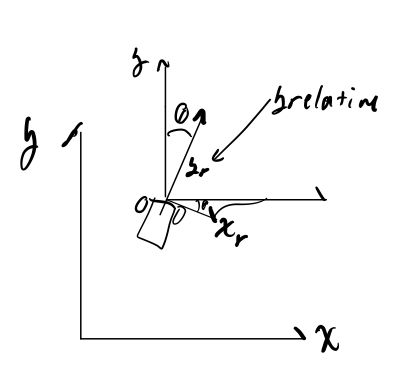
\includegraphics[scale=.75]{axis}\\
The value $\theta$ shall be defined as the angle between the absolute axis $y$ and the relative axis $y_{r}$. Thus if directional velocity is represented by $\frac{dy}{dt}$ and $\frac{dx}{dt}$ we can say that:\\\\
$dy = dy_r cos(\theta) - dx_r sin(\theta)$\\\\
$dx = dy_r sin(\theta) + dx_r cos(\theta)$\\\\
\subsection{Defining movement based on rotational velocity.}
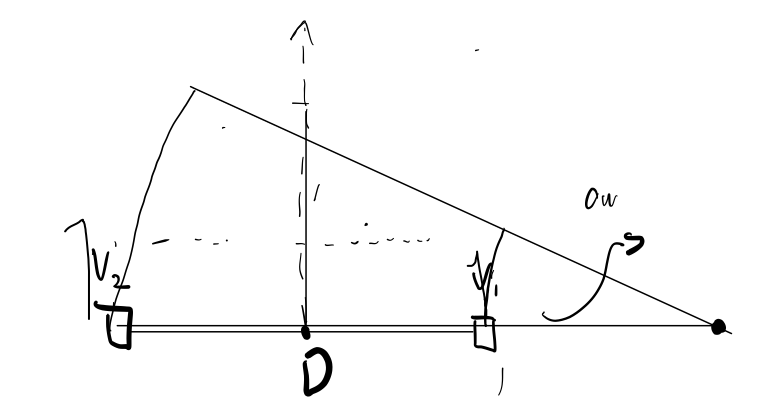
\includegraphics[scale=.75]{rotate.png}\\
Should we imagine that the angular velocities of the wheels $\omega_{1}$ and $\omega_{2}$ are not equal the car would follow an arched path rotating along an arbitrary axis. \\
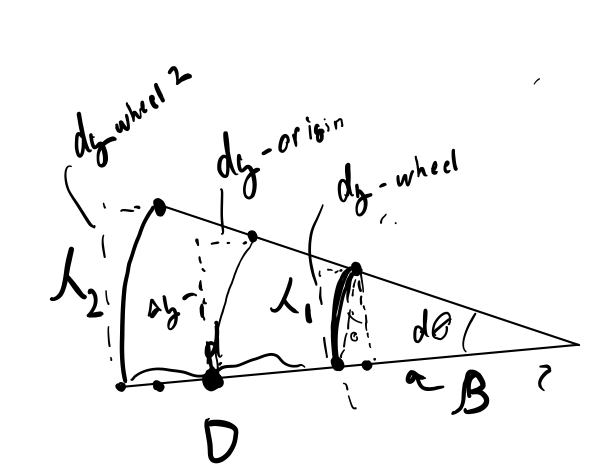
\includegraphics[scale=.75]{rotatediff.png}\\
We can then define a differential distances $\lambda_{1} = \omega_{1} r dt$ and $\lambda_{2} =\omega_{1} r dt$ (where $r$ is the radius of the wheel) representing the differential arched distance each wheel travels and $d\theta$ representing the differential change in angle of the device. $D$ represents the width of the vehicle and $\beta$ represents the distance between the right wheel and the temporary axis of rotation. We thus we can say:\\\\
$d\theta*\beta = \lambda_{1}$\\
$d\theta*(\beta + D) = \lambda_{2}$\\
$d\theta= \frac{\lambda_{2} - \lambda_{1}}{D}$\\
Thus:\\\\
\boldmath$\frac{d\theta}{dt}= \frac{\omega_{2}r - \omega_{1}r}{D}$\unboldmath\\\\\\
Now $dy_r$ is the average of the change in distances of the wheels $dy_{1}$ and $dy_{2}$. Since this forms an arbitrary unit circle, we can easily say:$dy_{1} = \beta sin(d\theta) = \frac{\lambda_{1}}{d\theta} sin(d\theta)$ and $dy_{2} = \frac{\lambda_{2}}{d\theta} sin(d\theta)$ thus $dy_r = \frac{\lambda_{2}+\lambda_{1}}{2d\theta} sin(d\theta)$. We can then substitute in $d\theta$ as defined above, and replace $\lambda$ with $\omega r$ to yield the resulting final equations:\\\\

$dy_r = \frac{D}{2}\frac{\omega_{2}+\omega_{1}}{\omega_{2}-\omega_{1}} sin(\frac{\omega_1 - \omega_2}{D}rdt)$\\\\

$dx_r = \frac{D}{2}\frac{\omega_{2}+\omega_{1}}{\omega_{2}-\omega_{1}} (1 - cos(\frac{\omega_1 - \omega_2}{D}rdt))$\\\\
If $\omega_{2}-\omega_{1} \neq 0$. If $\omega_{2}-\omega_{1} = 0$ we will end up dividing 0 by 0, thus we must take the limit as this difference approaches 0 which yields:\\\\
$dy_r = r\omega_1 = r\omega_2$\\
$dx_r =0$\\\\
If $\omega_{2}-\omega_{1} = 0$. This intuitively makes sense. Also if $\omega_1 = \omega_2$ then both distances would be 0, which also checks out since this would be the condition where the cart is simply spinning in a circle. To obtain change in absolute position one must simply plug in these relative equations into the aforementioned relative equation. So once again:\\
\[
    dy_r= 
\begin{cases}
    \frac{D}{2}\frac{\omega_{2}+\omega_{1}}{\omega_{2}-\omega_{1}} sin(\frac{\omega_1 - \omega_2}{D}rdt),& \text{if } \omega_{2}-\omega_{1} \neq 0\\
    r\omega_1 = r\omega_2,              & \text{otherwise}
\end{cases}
\]

\[
    dx_r= 
\begin{cases}
    \frac{D}{2}\frac{\omega_{2}+\omega_{1}}{\omega_{2}-\omega_{1}} (1 - cos(\frac{\omega_1 - \omega_2}{D}rdt)),& \text{if } \omega_{2}-\omega_{1} \neq 0\\
    0,              & \text{otherwise}
\end{cases}
\]\\
$dy = dy_r cos(\theta) - dx_r sin(\theta)$\\
$dx = dy_r sin(\theta) + dx_r cos(\theta)$\\\\
$d\theta= \frac{\omega_{2}r - \omega_{1}r}{D} dt$




\end{document}